\documentclass[letterpaper, 10pt]{article}

\usepackage[a3paper, margin = 0.25in]{geometry}
\usepackage{tikz}
\usepackage{xcolor}
\usepackage{multicol}
\usepackage{import}

\pagestyle{empty}

\definecolor{vblack}{HTML}{1A1A1A}
\definecolor{vgray}{HTML}{686868}
\definecolor{vblue}{HTML}{007acc}

\def\one{
	\draw[draw = vblue, fill = vblue] (-.6,.1) circle (.05);
	\draw [draw = none, fill = vblue] (-.65,.1) -- (-.6,.25) -- (-.55,.1) -- cycle;	
}
\def\two{
	\draw[draw = vblue, fill = vblue] (-.4,.1) circle (.05);
	\draw [draw = none, fill = vblue] (-.45,.1) -- (-.4,.25) -- (-.35,.1) -- cycle;
}
\def\three{
	\draw[draw = vblue, fill = vblue] (-.2,.1) circle (.05);
	\draw [draw = none, fill = vblue] (-.25,.1) -- (-.2,.25) -- (-.15,.1) -- cycle;
}
\def\four{
	\draw[draw = vblue, fill = vblue] (0,.1) circle (.05);
	\draw [draw = none, fill = vblue] (-.05,.1) -- (0,.25) -- (.05,.1) -- cycle;
}
\def\five{
	\draw[draw = vblue, fill = vblue] (.4,.1) circle (.05);
	\draw [draw = none, fill = vblue] (.35,.1) -- (.4,.25) -- (.45,.1) -- cycle;
}
\def\six{
	\draw[draw = vblue, fill = vblue] (.6,.1) circle (.05);
	\draw [draw = none, fill = vblue] (.55,.1) -- (.6,.25) -- (.65,.1) -- cycle;
}
\def\seven{
	\draw[draw = vblue, fill = vblue] (.8,.1) circle (.05);
	\draw [draw = none, fill = vblue] (.75,.1) -- (.8,.25) -- (.85,.1) -- cycle;
}
\def\eight{
	\draw[draw = vblue, fill = vblue] (1,.1) circle (.05);
	\draw [draw = none, fill = vblue] (.95,.1) -- (1,.25) -- (1.05,.1) -- cycle;
}
\def\gone{
	\draw[draw = vgray, fill = vgray] (-.6,.1) circle (.05);
	\draw [draw = none, fill = vgray] (-.65,.1) -- (-.6,.25) -- (-.55,.1) -- cycle;	
}
\def\gtwo{
	\draw[draw = vgray, fill = vgray] (-.4,.1) circle (.05);
	\draw [draw = none, fill = vgray] (-.45,.1) -- (-.4,.25) -- (-.35,.1) -- cycle;
}
\def\gthree{
	\draw[draw = vgray, fill = vgray] (-.2,.1) circle (.05);
	\draw [draw = none, fill = vgray] (-.25,.1) -- (-.2,.25) -- (-.15,.1) -- cycle;
}
\def\gfour{
	\draw[draw = vgray, fill = vgray] (0,.1) circle (.05);
	\draw [draw = none, fill = vgray] (-.05,.1) -- (0,.25) -- (.05,.1) -- cycle;
}
\def\gfive{
	\draw[draw = vgray, fill = vgray] (.4,.1) circle (.05);
	\draw [draw = none, fill = vgray] (.35,.1) -- (.4,.25) -- (.45,.1) -- cycle;
}
\def\gsix{
	\draw[draw = vgray, fill = vgray] (.6,.1) circle (.05);
	\draw [draw = none, fill = vgray] (.55,.1) -- (.6,.25) -- (.65,.1) -- cycle;
}
\def\gseven{
	\draw[draw = vgray, fill = vgray] (.8,.1) circle (.05);
	\draw [draw = none, fill = vgray] (.75,.1) -- (.8,.25) -- (.85,.1) -- cycle;
}
\def\geight{
	\draw[draw = vgray, fill = vgray] (1,.1) circle (.05);
	\draw [draw = none, fill = vgray] (.95,.1) -- (1,.25) -- (1.05,.1) -- cycle;
}

\def\othree{
	\draw[draw = orange, fill = orange] (-.2,.1) circle (.05);
	\draw [draw = none, fill = orange] (-.25,.1) -- (-.2,.25) -- (-.15,.1) -- cycle;
}
\def\ofive{
	\draw[draw = orange, fill = orange] (.4,.1) circle (.05);
	\draw [draw = none, fill = orange] (.35,.1) -- (.4,.25) -- (.45,.1) -- cycle;
}
\def\oeight{
	\draw[draw = orange, fill = orange] (1,.1) circle (.05);
	\draw [draw = none, fill = orange] (.95,.1) -- (1,.25) -- (1.05,.1) -- cycle;
}

\def\menorah#1{
	\draw[draw = vblack] (0,0) arc(180:360:.2);
	\draw[draw = vblack] (-.2,0) arc(180:360:.4);
	\draw[draw = vblack] (-.4,0) arc(180:360:.6);
	\draw[draw = vblack] (-.6,0) arc(180:360:.8);
	\draw[draw = vblack] (.2,-1) -- (.2,.2);
	\draw[draw = vblue, fill = vblue] (.2,.3) circle (.05);
	\draw[draw = none, fill = vblue] (.15,.3) -- (.2,.45) -- (.25, .3) -- cycle;
	\draw (-1.25,-.25) node{\ $#1$};
	\draw (1.75,.25) node{};
	\draw (-1.75,.25) node{};
}

\def\gmenorah#1{
	\draw[draw = vblack] (0,0) arc(180:360:.2);
	\draw[draw = vblack] (-.2,0) arc(180:360:.4);
	\draw[draw = vblack] (-.4,0) arc(180:360:.6);
	\draw[draw = vblack] (-.6,0) arc(180:360:.8);
	\draw[draw = vblack] (.2,-1) -- (.2,.2);
	\draw[draw = vgray, fill = vgray] (.2,.3) circle (.05);
	\draw[draw = none, fill = vgray] (.15,.3) -- (.2,.45) -- (.25, .3) -- cycle;
	\draw (-1.25,-.25) node{\ $#1$};
	\draw (1.75,.25) node{};
	\draw (-1.75,.25) node{};
}

\begin{document}
	\begin{multicols}{8}\noindent
		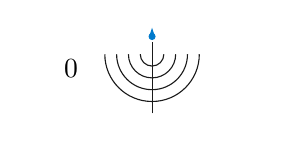
\begin{tikzpicture}[scale = 0.75]
	\menorah{0}
	
\end{tikzpicture}
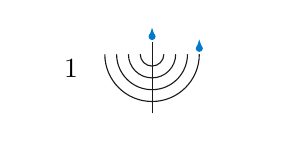
\begin{tikzpicture}[scale = 0.75]
	\menorah{1}
	\eight
\end{tikzpicture}
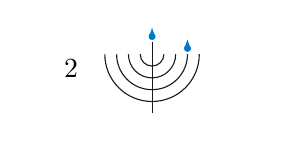
\begin{tikzpicture}[scale = 0.75]
	\menorah{2}
	\seven
\end{tikzpicture}
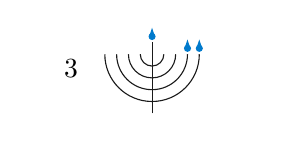
\begin{tikzpicture}[scale = 0.75]
	\menorah{3}
	\seven\eight
\end{tikzpicture}
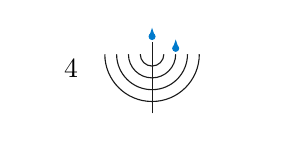
\begin{tikzpicture}[scale = 0.75]
	\menorah{4}
	\six
\end{tikzpicture}
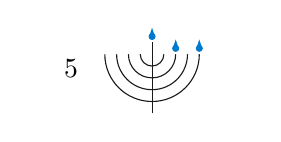
\begin{tikzpicture}[scale = 0.75]
	\menorah{5}
	\six\eight
\end{tikzpicture}
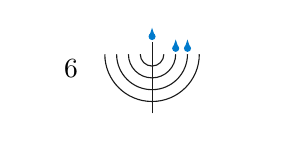
\begin{tikzpicture}[scale = 0.75]
	\menorah{6}
	\six\seven
\end{tikzpicture}
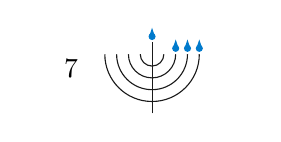
\begin{tikzpicture}[scale = 0.75]
	\menorah{7}
	\six\seven\eight
\end{tikzpicture}
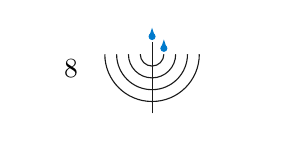
\begin{tikzpicture}[scale = 0.75]
	\menorah{8}
	\five
\end{tikzpicture}
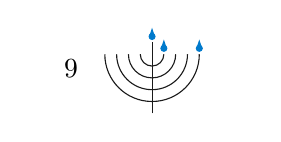
\begin{tikzpicture}[scale = 0.75]
	\menorah{9}
	\five\eight
\end{tikzpicture}
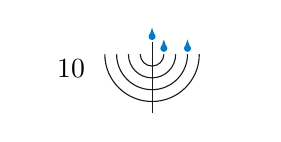
\begin{tikzpicture}[scale = 0.75]
	\menorah{10}
	\five\seven
\end{tikzpicture}
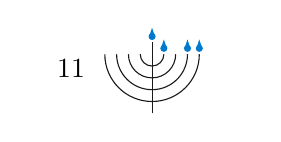
\begin{tikzpicture}[scale = 0.75]
	\menorah{11}
	\five\seven\eight
\end{tikzpicture}
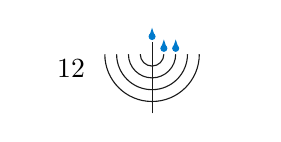
\begin{tikzpicture}[scale = 0.75]
	\menorah{12}
	\five\six
\end{tikzpicture}
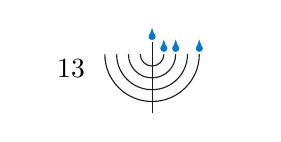
\begin{tikzpicture}[scale = 0.75]
	\menorah{13}
	\five\six\eight
\end{tikzpicture}
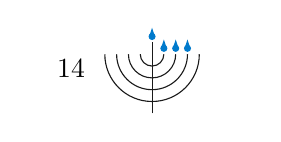
\begin{tikzpicture}[scale = 0.75]
	\menorah{14}
	\five\six\seven
\end{tikzpicture}
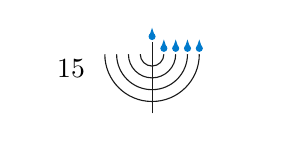
\begin{tikzpicture}[scale = 0.75]
	\menorah{15}
	\five\six\seven\eight
\end{tikzpicture}
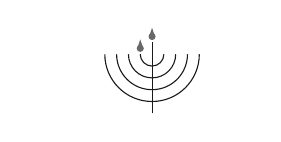
\begin{tikzpicture}[scale = 0.75]
	\gmenorah{}
	\gfour
\end{tikzpicture}
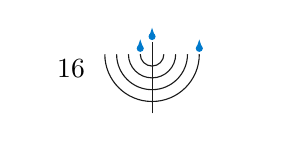
\begin{tikzpicture}[scale = 0.75]
	\menorah{16}
	\four\eight
\end{tikzpicture}
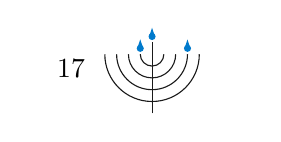
\begin{tikzpicture}[scale = 0.75]
	\menorah{17}
	\four\seven
\end{tikzpicture}
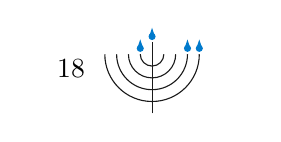
\begin{tikzpicture}[scale = 0.75]
	\menorah{18}
	\four\seven\eight
\end{tikzpicture}
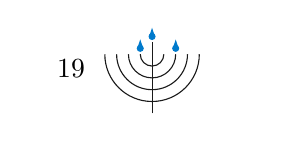
\begin{tikzpicture}[scale = 0.75]
	\menorah{19}
	\four\six
\end{tikzpicture}
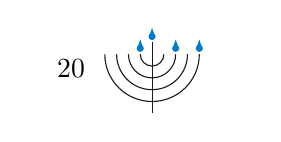
\begin{tikzpicture}[scale = 0.75]
	\menorah{20}
	\four\six\eight
\end{tikzpicture}
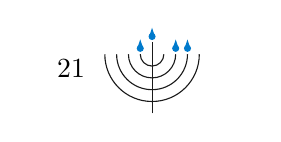
\begin{tikzpicture}[scale = 0.75]
	\menorah{21}
	\four\six\seven
\end{tikzpicture}
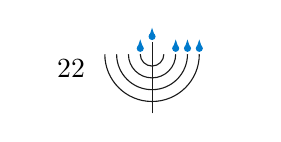
\begin{tikzpicture}[scale = 0.75]
	\menorah{22}
	\four\six\seven\eight
\end{tikzpicture}
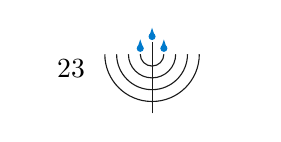
\begin{tikzpicture}[scale = 0.75]
	\menorah{23}
	\four\five
\end{tikzpicture}
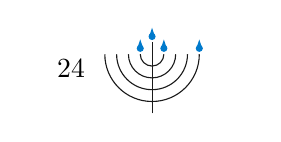
\begin{tikzpicture}[scale = 0.75]
	\menorah{24}
	\four\five\eight
\end{tikzpicture}
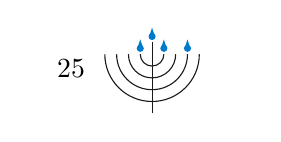
\begin{tikzpicture}[scale = 0.75]
	\menorah{25}
	\four\five\seven
\end{tikzpicture}
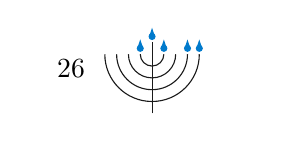
\begin{tikzpicture}[scale = 0.75]
	\menorah{26}
	\four\five\seven\eight
\end{tikzpicture}
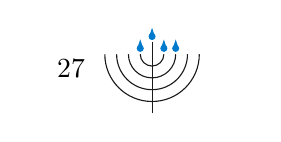
\begin{tikzpicture}[scale = 0.75]
	\menorah{27}
	\four\five\six
\end{tikzpicture}
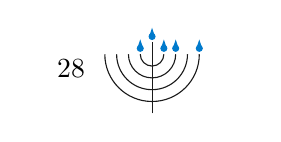
\begin{tikzpicture}[scale = 0.75]
	\menorah{28}
	\four\five\six\eight
\end{tikzpicture}
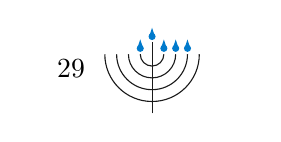
\begin{tikzpicture}[scale = 0.75]
	\menorah{29}
	\four\five\six\seven
\end{tikzpicture}
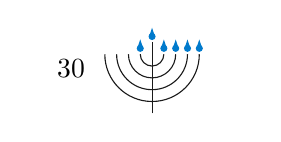
\begin{tikzpicture}[scale = 0.75]
	\menorah{30}
	\four\five\six\seven\eight
\end{tikzpicture}
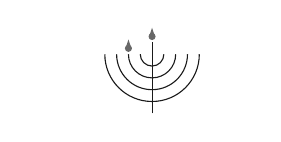
\begin{tikzpicture}[scale = 0.75]
	\gmenorah{}
	\gthree
\end{tikzpicture}
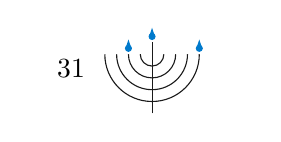
\begin{tikzpicture}[scale = 0.75]
	\menorah{31}
	\three\eight
\end{tikzpicture}
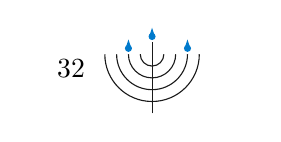
\begin{tikzpicture}[scale = 0.75]
	\menorah{32}
	\three\seven
\end{tikzpicture}
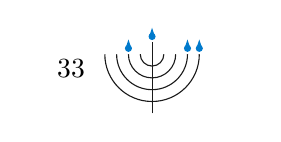
\begin{tikzpicture}[scale = 0.75]
	\menorah{33}
	\three\seven\eight
\end{tikzpicture}
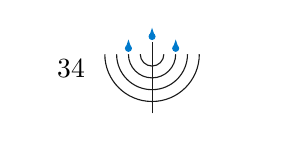
\begin{tikzpicture}[scale = 0.75]
	\menorah{34}
	\three\six
\end{tikzpicture}
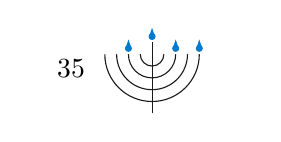
\begin{tikzpicture}[scale = 0.75]
	\menorah{35}
	\three\six\eight
\end{tikzpicture}
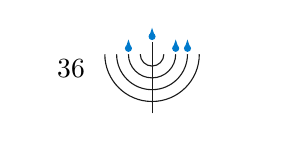
\begin{tikzpicture}[scale = 0.75]
	\menorah{36}
	\three\six\seven
\end{tikzpicture}
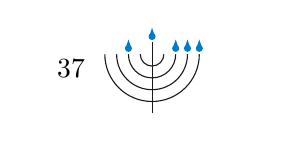
\begin{tikzpicture}[scale = 0.75]
	\menorah{37}
	\three\six\seven\eight
\end{tikzpicture}
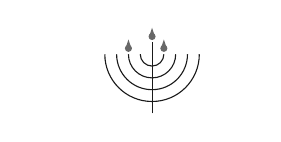
\begin{tikzpicture}[scale = 0.75]
	\gmenorah{}
	\gthree\gfive
\end{tikzpicture}
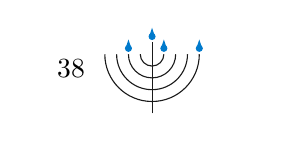
\begin{tikzpicture}[scale = 0.75]
	\menorah{38}
	\three\five\eight
\end{tikzpicture}
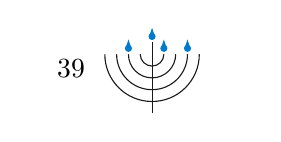
\begin{tikzpicture}[scale = 0.75]
	\menorah{39}
	\three\five\seven
\end{tikzpicture}
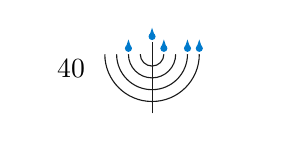
\begin{tikzpicture}[scale = 0.75]
	\menorah{40}
	\three\five\seven\eight
\end{tikzpicture}
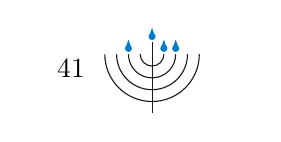
\begin{tikzpicture}[scale = 0.75]
	\menorah{41}
	\three\five\six
\end{tikzpicture}
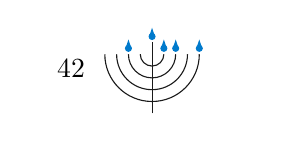
\begin{tikzpicture}[scale = 0.75]
	\menorah{42}
	\three\five\six\eight
\end{tikzpicture}
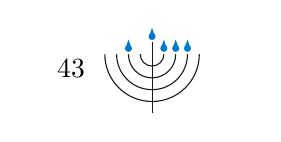
\begin{tikzpicture}[scale = 0.75]
	\menorah{43}
	\three\five\six\seven
\end{tikzpicture}
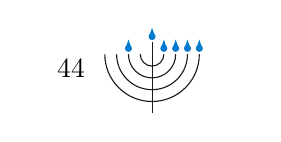
\begin{tikzpicture}[scale = 0.75]
	\menorah{44}
	\three\five\six\seven\eight
\end{tikzpicture}
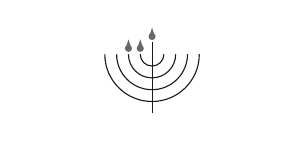
\begin{tikzpicture}[scale = 0.75]
	\gmenorah{}
	\gthree\gfour
\end{tikzpicture}
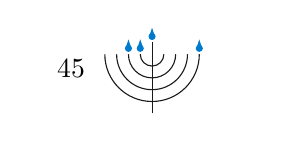
\begin{tikzpicture}[scale = 0.75]
	\menorah{45}
	\three\four\eight
\end{tikzpicture}
\begin{tikzpicture}[scale = 0.75]
	\menorah{46}
	\three\four\seven
\end{tikzpicture}
\begin{tikzpicture}[scale = 0.75]
	\menorah{47}
	\three\four\seven\eight
\end{tikzpicture}
\begin{tikzpicture}[scale = 0.75]
	\gmenorah{}
	\gthree\gfour\gsix
\end{tikzpicture}
\begin{tikzpicture}[scale = 0.75]
	\menorah{48}
	\three\four\six\eight
\end{tikzpicture}
\begin{tikzpicture}[scale = 0.75]
	\menorah{49}
	\three\four\six\seven
\end{tikzpicture}
\begin{tikzpicture}[scale = 0.75]
	\menorah{50}
	\three\four\six\seven\eight
\end{tikzpicture}
\begin{tikzpicture}[scale = 0.75]
	\gmenorah{}
	\gthree\gfour\gfive
\end{tikzpicture}
\begin{tikzpicture}[scale = 0.75]
	\menorah{51}
	\three\four\five\eight
\end{tikzpicture}
\begin{tikzpicture}[scale = 0.75]
	\menorah{52}
	\three\four\five\seven
\end{tikzpicture}
\begin{tikzpicture}[scale = 0.75]
	\menorah{53}
	\three\four\five\seven\eight
\end{tikzpicture}
\begin{tikzpicture}[scale = 0.75]
	\menorah{54}
	\three\four\five\six
\end{tikzpicture}
\begin{tikzpicture}[scale = 0.75]
	\menorah{55}
	\three\four\five\six\eight
\end{tikzpicture}
\begin{tikzpicture}[scale = 0.75]
	\menorah{56}
	\three\four\five\six\seven
\end{tikzpicture}
\begin{tikzpicture}[scale = 0.75]
	\menorah{57}
	\three\four\five\six\seven\eight
\end{tikzpicture}
\begin{tikzpicture}[scale = 0.75]
	\gmenorah{}
	\gtwo
\end{tikzpicture}
\begin{tikzpicture}[scale = 0.75]
	\menorah{58}
	\two\eight
\end{tikzpicture}
\begin{tikzpicture}[scale = 0.75]
	\menorah{59}
	\two\seven
\end{tikzpicture}
\begin{tikzpicture}[scale = 0.75]
	\menorah{60}
	\two\seven\eight
\end{tikzpicture}
\begin{tikzpicture}[scale = 0.75]
	\gmenorah{}
	\gtwo\gsix
\end{tikzpicture}
\begin{tikzpicture}[scale = 0.75]
	\menorah{61}
	\two\six\eight
\end{tikzpicture}
\begin{tikzpicture}[scale = 0.75]
	\menorah{62}
	\two\six\seven
\end{tikzpicture}
\begin{tikzpicture}[scale = 0.75]
	\menorah{63}
	\two\six\seven\eight
\end{tikzpicture}
\begin{tikzpicture}[scale = 0.75]
	\gmenorah{}
	\gtwo\gfive
\end{tikzpicture}
\begin{tikzpicture}[scale = 0.75]
	\menorah{64}
	\two\five\eight
\end{tikzpicture}
\begin{tikzpicture}[scale = 0.75]
	\menorah{65}
	\two\five\seven
\end{tikzpicture}
\begin{tikzpicture}[scale = 0.75]
	\menorah{66}
	\two\five\seven\eight
\end{tikzpicture}
\begin{tikzpicture}[scale = 0.75]
	\gmenorah{}
	\gtwo\gfive\gsix
\end{tikzpicture}
\begin{tikzpicture}[scale = 0.75]
	\menorah{67}
	\two\five\six\eight
\end{tikzpicture}
\begin{tikzpicture}[scale = 0.75]
	\menorah{68}
	\two\five\six\seven
\end{tikzpicture}
\begin{tikzpicture}[scale = 0.75]
	\menorah{69}
	\two\five\six\seven\eight
\end{tikzpicture}
\begin{tikzpicture}[scale = 0.75]
	\gmenorah{}
	\gtwo\gfour
\end{tikzpicture}
\begin{tikzpicture}[scale = 0.75]
	\menorah{70}
	\two\four\eight
\end{tikzpicture}
\begin{tikzpicture}[scale = 0.75]
	\gmenorah{}
	\gtwo\gfour\gseven
\end{tikzpicture}
\begin{tikzpicture}[scale = 0.75]
	\menorah{71}
	\two\four\seven\eight
\end{tikzpicture}
\begin{tikzpicture}[scale = 0.75]
	\gmenorah{}
	\gtwo\gfour\gsix
\end{tikzpicture}
\begin{tikzpicture}[scale = 0.75]
	\menorah{72}
	\two\four\six\eight
\end{tikzpicture}
\begin{tikzpicture}[scale = 0.75]
	\menorah{73}
	\two\four\six\seven
\end{tikzpicture}
\begin{tikzpicture}[scale = 0.75]
	\menorah{74}
	\two\four\six\seven\eight
\end{tikzpicture}
\begin{tikzpicture}[scale = 0.75]
	\gmenorah{}
	\gtwo\gfour\gfive
\end{tikzpicture}
\begin{tikzpicture}[scale = 0.75]
	\menorah{75}
	\two\four\five\eight
\end{tikzpicture}
\begin{tikzpicture}[scale = 0.75]
	\menorah{76}
	\two\four\five\seven
\end{tikzpicture}
\begin{tikzpicture}[scale = 0.75]
	\menorah{77}
	\two\four\five\seven\eight
\end{tikzpicture}
\begin{tikzpicture}[scale = 0.75]
	\gmenorah{}
	\gtwo\gfour\gfive\gsix
\end{tikzpicture}
\begin{tikzpicture}[scale = 0.75]
	\menorah{78}
	\two\four\five\six\eight
\end{tikzpicture}
\begin{tikzpicture}[scale = 0.75]
	\menorah{79}
	\two\four\five\six\seven
\end{tikzpicture}
\begin{tikzpicture}[scale = 0.75]
	\menorah{80}
	\two\four\five\six\seven\eight
\end{tikzpicture}
\begin{tikzpicture}[scale = 0.75]
	\gmenorah{}
	\gtwo\gthree
\end{tikzpicture}
\begin{tikzpicture}[scale = 0.75]
	\menorah{81}
	\two\three\eight
\end{tikzpicture}
\begin{tikzpicture}[scale = 0.75]
	\gmenorah{}
	\gtwo\gthree\gseven
\end{tikzpicture}
\begin{tikzpicture}[scale = 0.75]
	\menorah{82}
	\two\three\seven\eight
\end{tikzpicture}
\begin{tikzpicture}[scale = 0.75]
	\gmenorah{}
	\gtwo\gthree\gsix
\end{tikzpicture}
\begin{tikzpicture}[scale = 0.75]
	\menorah{83}
	\two\three\six\eight
\end{tikzpicture}
\begin{tikzpicture}[scale = 0.75]
	\menorah{84}
	\two\three\six\seven
\end{tikzpicture}
\begin{tikzpicture}[scale = 0.75]
	\menorah{85}
	\two\three\six\seven\eight
\end{tikzpicture}
\begin{tikzpicture}[scale = 0.75]
	\gmenorah{}
	\gtwo\gthree\gfive
\end{tikzpicture}
\begin{tikzpicture}[scale = 0.75]
	\menorah{86}
	\two\three\five\eight
\end{tikzpicture}
\begin{tikzpicture}[scale = 0.75]
	\gmenorah{}
	\gtwo\gthree\gfive\gseven
\end{tikzpicture}
\begin{tikzpicture}[scale = 0.75]
	\menorah{87}
	\two\three\five\seven\eight
\end{tikzpicture}
\begin{tikzpicture}[scale = 0.75]
	\gmenorah{}
	\gtwo\gthree\gfive\gsix
\end{tikzpicture}
\begin{tikzpicture}[scale = 0.75]
	\menorah{88}
	\two\three\five\six\eight
\end{tikzpicture}
\begin{tikzpicture}[scale = 0.75]
	\menorah{89}
	\two\three\five\six\seven
\end{tikzpicture}
\begin{tikzpicture}[scale = 0.75]
	\menorah{90}
	\two\three\five\six\seven\eight
\end{tikzpicture}
\begin{tikzpicture}[scale = 0.75]
	\gmenorah{}
	\gtwo\gthree\gfour
\end{tikzpicture}
\begin{tikzpicture}[scale = 0.75]
	\menorah{91}
	\two\three\four\eight
\end{tikzpicture}
\begin{tikzpicture}[scale = 0.75]
	\gmenorah{}
	\gtwo\gthree\gfour\gseven
\end{tikzpicture}
\begin{tikzpicture}[scale = 0.75]
	\menorah{92}
	\two\three\four\seven\eight
\end{tikzpicture}
\begin{tikzpicture}[scale = 0.75]
	\gmenorah{}
	\gtwo\gthree\gfour\gsix
\end{tikzpicture}
\begin{tikzpicture}[scale = 0.75]
	\menorah{93}
	\two\three\four\six\eight
\end{tikzpicture}
\begin{tikzpicture}[scale = 0.75]
	\gmenorah{}
	\gtwo\gthree\gfour\gsix\gseven
\end{tikzpicture}
\begin{tikzpicture}[scale = 0.75]
	\menorah{94}
	\two\three\four\six\seven\eight
\end{tikzpicture}
\begin{tikzpicture}[scale = 0.75]
	\gmenorah{}
	\gtwo\gthree\gfour\gfive
\end{tikzpicture}
\begin{tikzpicture}[scale = 0.75]
	\menorah{95}
	\two\three\four\five\eight
\end{tikzpicture}
\begin{tikzpicture}[scale = 0.75]
	\gmenorah{}
	\gtwo\gthree\gfour\gfive\gseven
\end{tikzpicture}
\begin{tikzpicture}[scale = 0.75]
	\menorah{96}
	\two\three\four\five\seven\eight
\end{tikzpicture}
\begin{tikzpicture}[scale = 0.75]
	\gmenorah{}
	\gtwo\gthree\gfour\gfive\gsix
\end{tikzpicture}
\begin{tikzpicture}[scale = 0.75]
	\menorah{97}
	\two\three\four\five\six\eight
\end{tikzpicture}
\begin{tikzpicture}[scale = 0.75]
	\menorah{98}
	\two\three\four\five\six\seven
\end{tikzpicture}
\begin{tikzpicture}[scale = 0.75]
	\menorah{99}
	\two\three\four\five\six\seven\eight
\end{tikzpicture}
\begin{tikzpicture}[scale = 0.75]
	\gmenorah{}
	\gone
\end{tikzpicture}
\begin{tikzpicture}[scale = 0.75]
	\menorah{100}
	\one\eight
\end{tikzpicture}
\begin{tikzpicture}[scale = 0.75]
	\gmenorah{}
	\gone\gseven
\end{tikzpicture}
\begin{tikzpicture}[scale = 0.75]
	\menorah{101}
	\one\seven\eight
\end{tikzpicture}
\begin{tikzpicture}[scale = 0.75]
	\gmenorah{}
	\gone\gsix
\end{tikzpicture}
\begin{tikzpicture}[scale = 0.75]
	\menorah{102}
	\one\six\eight
\end{tikzpicture}
\begin{tikzpicture}[scale = 0.75]
	\gmenorah{}
	\gone\gsix\gseven
\end{tikzpicture}
\begin{tikzpicture}[scale = 0.75]
	\menorah{103}
	\one\six\seven\eight
\end{tikzpicture}
\begin{tikzpicture}[scale = 0.75]
	\gmenorah{}
	\gone\gfive
\end{tikzpicture}
\begin{tikzpicture}[scale = 0.75]
	\menorah{104}
	\one\five\eight
\end{tikzpicture}
\begin{tikzpicture}[scale = 0.75]
	\gmenorah{}
	\gone\gfive\gseven
\end{tikzpicture}
\begin{tikzpicture}[scale = 0.75]
	\menorah{105}
	\one\five\seven\eight
\end{tikzpicture}
\begin{tikzpicture}[scale = 0.75]
	\gmenorah{}
	\gone\gfive\gsix
\end{tikzpicture}
\begin{tikzpicture}[scale = 0.75]
	\menorah{106}
	\one\five\six\eight
\end{tikzpicture}
\begin{tikzpicture}[scale = 0.75]
	\gmenorah{}
	\gone\gfive\gsix\gseven
\end{tikzpicture}
\begin{tikzpicture}[scale = 0.75]
	\menorah{107}
	\one\five\six\seven\eight
\end{tikzpicture}
\begin{tikzpicture}[scale = 0.75]
	\gmenorah{}
	\gone\gfour
\end{tikzpicture}
\begin{tikzpicture}[scale = 0.75]
	\gmenorah{}
	\gone\gfour\geight
\end{tikzpicture}
\begin{tikzpicture}[scale = 0.75]
	\gmenorah{}
	\gone\gfour\gseven
\end{tikzpicture}
\begin{tikzpicture}[scale = 0.75]
	\menorah{108}
	\one\four\seven\eight
\end{tikzpicture}
\begin{tikzpicture}[scale = 0.75]
	\gmenorah{}
	\gone\gfour\gsix
\end{tikzpicture}
\begin{tikzpicture}[scale = 0.75]
	\menorah{109}
	\one\four\six\eight
\end{tikzpicture}
\begin{tikzpicture}[scale = 0.75]
	\gmenorah{}
	\gone\gfour\gsix\gseven
\end{tikzpicture}
\begin{tikzpicture}[scale = 0.75]
	\menorah{110}
	\one\four\six\seven\eight
\end{tikzpicture}
\begin{tikzpicture}[scale = 0.75]
	\gmenorah{}
	\gone\gfour\gfive
\end{tikzpicture}
\begin{tikzpicture}[scale = 0.75]
	\menorah{111}
	\one\four\five\eight
\end{tikzpicture}
\begin{tikzpicture}[scale = 0.75]
	\gmenorah{}
	\gone\gfour\gfive\gseven
\end{tikzpicture}
\begin{tikzpicture}[scale = 0.75]
	\menorah{112}
	\one\four\five\seven\eight
\end{tikzpicture}
\begin{tikzpicture}[scale = 0.75]
	\gmenorah{}
	\gone\gfour\gfive\gsix
\end{tikzpicture}
\begin{tikzpicture}[scale = 0.75]
	\menorah{113}
	\one\four\five\six\eight
\end{tikzpicture}
\begin{tikzpicture}[scale = 0.75]
	\gmenorah{}
	\gone\gfour\gfive\gsix\gseven
\end{tikzpicture}
\begin{tikzpicture}[scale = 0.75]
	\menorah{114}
	\one\four\five\six\seven\eight
\end{tikzpicture}
\begin{tikzpicture}[scale = 0.75]
	\gmenorah{}
	\gone\gthree
\end{tikzpicture}
\begin{tikzpicture}[scale = 0.75]
	\gmenorah{}
	\gone\gthree\geight
\end{tikzpicture}
\begin{tikzpicture}[scale = 0.75]
	\gmenorah{}
	\gone\gthree\gseven
\end{tikzpicture}
\begin{tikzpicture}[scale = 0.75]
	\menorah{115}
	\one\three\seven\eight
\end{tikzpicture}
\begin{tikzpicture}[scale = 0.75]
	\gmenorah{}
	\gone\gthree\gsix
\end{tikzpicture}
\begin{tikzpicture}[scale = 0.75]
	\menorah{116}
	\one\three\six\eight
\end{tikzpicture}
\begin{tikzpicture}[scale = 0.75]
	\gmenorah{}
	\gone\gthree\gsix\gseven
\end{tikzpicture}
\begin{tikzpicture}[scale = 0.75]
	\menorah{117}
	\one\three\six\seven\eight
\end{tikzpicture}
\begin{tikzpicture}[scale = 0.75]
	\gmenorah{}
	\gone\gthree\gfive
\end{tikzpicture}
\begin{tikzpicture}[scale = 0.75]
	\gmenorah{}
	\gone\gthree\gfive\geight
\end{tikzpicture}
\begin{tikzpicture}[scale = 0.75]
	\gmenorah{}
	\gone\gthree\gfive\gseven
\end{tikzpicture}
\begin{tikzpicture}[scale = 0.75]
	\menorah{118}
	\one\three\five\seven\eight
\end{tikzpicture}
\begin{tikzpicture}[scale = 0.75]
	\gmenorah{}
	\gone\gthree\gfive\gsix
\end{tikzpicture}
\begin{tikzpicture}[scale = 0.75]
	\menorah{119}
	\one\three\five\six\eight
\end{tikzpicture}
\begin{tikzpicture}[scale = 0.75]
	\gmenorah{}
	\gone\gthree\gfive\gsix\gseven
\end{tikzpicture}
\begin{tikzpicture}[scale = 0.75]
	\menorah{120}
	\one\three\five\six\seven\eight
\end{tikzpicture}
\begin{tikzpicture}[scale = 0.75]
	\gmenorah{}
	\gone\gthree\gfour
\end{tikzpicture}
\begin{tikzpicture}[scale = 0.75]
	\gmenorah{}
	\gone\gthree\gfour\geight
\end{tikzpicture}
\begin{tikzpicture}[scale = 0.75]
	\gmenorah{}
	\gone\gthree\gfour\gseven
\end{tikzpicture}
\begin{tikzpicture}[scale = 0.75]
	\menorah{121}
	\one\three\four\seven\eight
\end{tikzpicture}
\begin{tikzpicture}[scale = 0.75]
	\gmenorah{}
	\gone\gthree\gfour\gsix
\end{tikzpicture}
\begin{tikzpicture}[scale = 0.75]
	\gmenorah{}
	\gone\gthree\gfour\gsix\geight
\end{tikzpicture}
\begin{tikzpicture}[scale = 0.75]
	\gmenorah{}
	\gone\gthree\gfour\gsix\gseven
\end{tikzpicture}
\begin{tikzpicture}[scale = 0.75]
	\menorah{122}
	\one\three\four\six\seven\eight
\end{tikzpicture}
\begin{tikzpicture}[scale = 0.75]
	\gmenorah{}
	\gone\gthree\gfour\gfive
\end{tikzpicture}
\begin{tikzpicture}[scale = 0.75]
	\gmenorah{}
	\gone\gthree\gfour\gfive\geight
\end{tikzpicture}
\begin{tikzpicture}[scale = 0.75]
	\gmenorah{}
	\gone\gthree\gfour\gfive\gseven
\end{tikzpicture}
\begin{tikzpicture}[scale = 0.75]
	\menorah{123}
	\one\three\four\five\seven\eight
\end{tikzpicture}
\begin{tikzpicture}[scale = 0.75]
	\gmenorah{}
	\gone\gthree\gfour\gfive\gsix
\end{tikzpicture}
\begin{tikzpicture}[scale = 0.75]
	\menorah{124}
	\one\three\four\five\six\eight
\end{tikzpicture}
\begin{tikzpicture}[scale = 0.75]
	\gmenorah{}
	\gone\gthree\gfour\gfive\gsix\gseven
\end{tikzpicture}
\begin{tikzpicture}[scale = 0.75]
	\menorah{125}
	\one\three\four\five\six\seven\eight
\end{tikzpicture}
\begin{tikzpicture}[scale = 0.75]
	\gmenorah{}
	\gone\gtwo
\end{tikzpicture}
\begin{tikzpicture}[scale = 0.75]
	\gmenorah{}
	\gone\gtwo\geight
\end{tikzpicture}
\begin{tikzpicture}[scale = 0.75]
	\gmenorah{}
	\gone\gtwo\gseven
\end{tikzpicture}
\begin{tikzpicture}[scale = 0.75]
	\menorah{126}
	\one\two\seven\eight
\end{tikzpicture}
\begin{tikzpicture}[scale = 0.75]
	\gmenorah{}
	\gone\gtwo\gsix
\end{tikzpicture}
\begin{tikzpicture}[scale = 0.75]
	\gmenorah{}
	\gone\gtwo\gsix\geight
\end{tikzpicture}
\begin{tikzpicture}[scale = 0.75]
	\gmenorah{}
	\gone\gtwo\gsix\gseven
\end{tikzpicture}
\begin{tikzpicture}[scale = 0.75]
	\menorah{127}
	\one\two\six\seven\eight
\end{tikzpicture}
\begin{tikzpicture}[scale = 0.75]
	\gmenorah{}
	\gone\gtwo\gfive
\end{tikzpicture}
\begin{tikzpicture}[scale = 0.75]
	\gmenorah{}
	\gone\gtwo\gfive\geight
\end{tikzpicture}
\begin{tikzpicture}[scale = 0.75]
	\gmenorah{}
	\gone\gtwo\gfive\gseven
\end{tikzpicture}
\begin{tikzpicture}[scale = 0.75]
	\menorah{128}
	\one\two\five\seven\eight
\end{tikzpicture}
\begin{tikzpicture}[scale = 0.75]
	\gmenorah{}
	\gone\gtwo\gfive\gsix
\end{tikzpicture}
\begin{tikzpicture}[scale = 0.75]
	\gmenorah{}
	\gone\gtwo\gfive\gsix\geight
\end{tikzpicture}
\begin{tikzpicture}[scale = 0.75]
	\gmenorah{}
	\gone\gtwo\gfive\gsix\gseven
\end{tikzpicture}
\begin{tikzpicture}[scale = 0.75]
	\menorah{129}
	\one\two\five\six\seven\eight
\end{tikzpicture}
\begin{tikzpicture}[scale = 0.75]
	\gmenorah{}
	\gone\gtwo\gfour
\end{tikzpicture}
\begin{tikzpicture}[scale = 0.75]
	\gmenorah{}
	\gone\gtwo\gfour\geight
\end{tikzpicture}
\begin{tikzpicture}[scale = 0.75]
	\gmenorah{}
	\gone\gtwo\gfour\gseven
\end{tikzpicture}
\begin{tikzpicture}[scale = 0.75]
	\gmenorah{}
	\gone\gtwo\gfour\gseven\geight
\end{tikzpicture}
\begin{tikzpicture}[scale = 0.75]
	\gmenorah{}
	\gone\gtwo\gfour\gsix
\end{tikzpicture}
\begin{tikzpicture}[scale = 0.75]
	\gmenorah{}
	\gone\gtwo\gfour\gsix\geight
\end{tikzpicture}
\begin{tikzpicture}[scale = 0.75]
	\gmenorah{}
	\gone\gtwo\gfour\gsix\gseven
\end{tikzpicture}
\begin{tikzpicture}[scale = 0.75]
	\menorah{130}
	\one\two\four\six\seven\eight
\end{tikzpicture}
\begin{tikzpicture}[scale = 0.75]
	\gmenorah{}
	\gone\gtwo\gfour\gfive
\end{tikzpicture}
\begin{tikzpicture}[scale = 0.75]
	\gmenorah{}
	\gone\gtwo\gfour\gfive\geight
\end{tikzpicture}
\begin{tikzpicture}[scale = 0.75]
	\gmenorah{}
	\gone\gtwo\gfour\gfive\gseven
\end{tikzpicture}
\begin{tikzpicture}[scale = 0.75]
	\menorah{131}
	\one\two\four\five\seven\eight
\end{tikzpicture}
\begin{tikzpicture}[scale = 0.75]
	\gmenorah{}
	\gone\gtwo\gfour\gfive\gsix
\end{tikzpicture}
\begin{tikzpicture}[scale = 0.75]
	\gmenorah{}
	\gone\gtwo\gfour\gfive\gsix\geight
\end{tikzpicture}
\begin{tikzpicture}[scale = 0.75]
	\gmenorah{}
	\gone\gtwo\gfour\gfive\gsix\gseven
\end{tikzpicture}
\begin{tikzpicture}[scale = 0.75]
	\menorah{132}
	\one\two\four\five\six\seven\eight
\end{tikzpicture}
\begin{tikzpicture}[scale = 0.75]
	\gmenorah{}
	\gone\gtwo\gthree
\end{tikzpicture}
\begin{tikzpicture}[scale = 0.75]
	\gmenorah{}
	\gone\gtwo\gthree\geight
\end{tikzpicture}
\begin{tikzpicture}[scale = 0.75]
	\gmenorah{}
	\gone\gtwo\gthree\gseven
\end{tikzpicture}
\begin{tikzpicture}[scale = 0.75]
	\gmenorah{}
	\gone\gtwo\gthree\gseven\geight
\end{tikzpicture}
\begin{tikzpicture}[scale = 0.75]
	\gmenorah{}
	\gone\gtwo\gthree\gsix
\end{tikzpicture}
\begin{tikzpicture}[scale = 0.75]
	\gmenorah{}
	\gone\gtwo\gthree\gsix\geight
\end{tikzpicture}
\begin{tikzpicture}[scale = 0.75]
	\gmenorah{}
	\gone\gtwo\gthree\gsix\gseven
\end{tikzpicture}
\begin{tikzpicture}[scale = 0.75]
	\menorah{133}
	\one\two\three\six\seven\eight
\end{tikzpicture}
\begin{tikzpicture}[scale = 0.75]
	\gmenorah{}
	\gone\gtwo\gthree\gfive
\end{tikzpicture}
\begin{tikzpicture}[scale = 0.75]
	\gmenorah{}
	\gone\gtwo\gthree\gfive\geight
\end{tikzpicture}
\begin{tikzpicture}[scale = 0.75]
	\gmenorah{}
	\gone\gtwo\gthree\gfive\gseven
\end{tikzpicture}
\begin{tikzpicture}[scale = 0.75]
	\gmenorah{}
	\gone\gtwo\gthree\gfive\gseven\geight
\end{tikzpicture}
\begin{tikzpicture}[scale = 0.75]
	\gmenorah{}
	\gone\gtwo\gthree\gfive\gsix
\end{tikzpicture}
\begin{tikzpicture}[scale = 0.75]
	\gmenorah{}
	\gone\gtwo\gthree\gfive\gsix\geight
\end{tikzpicture}
\begin{tikzpicture}[scale = 0.75]
	\gmenorah{}
	\gone\gtwo\gthree\gfive\gsix\gseven
\end{tikzpicture}
\begin{tikzpicture}[scale = 0.75]
	\menorah{134}
	\one\two\three\five\six\seven\eight
\end{tikzpicture}
\begin{tikzpicture}[scale = 0.75]
	\gmenorah{}
	\gone\gtwo\gthree\gfour
\end{tikzpicture}
\begin{tikzpicture}[scale = 0.75]
	\gmenorah{}
	\gone\gtwo\gthree\gfour\geight
\end{tikzpicture}
\begin{tikzpicture}[scale = 0.75]
	\gmenorah{}
	\gone\gtwo\gthree\gfour\gseven
\end{tikzpicture}
\begin{tikzpicture}[scale = 0.75]
	\gmenorah{}
	\gone\gtwo\gthree\gfour\gseven\geight
\end{tikzpicture}
\begin{tikzpicture}[scale = 0.75]
	\gmenorah{}
	\gone\gtwo\gthree\gfour\gsix
\end{tikzpicture}
\begin{tikzpicture}[scale = 0.75]
	\gmenorah{}
	\gone\gtwo\gthree\gfour\gsix\geight
\end{tikzpicture}
\begin{tikzpicture}[scale = 0.75]
	\gmenorah{}
	\gone\gtwo\gthree\gfour\gsix\gseven
\end{tikzpicture}
\begin{tikzpicture}[scale = 0.75]
	\gmenorah{}
	\gone\gtwo\gthree\gfour\gsix\gseven\geight
\end{tikzpicture}
\begin{tikzpicture}[scale = 0.75]
	\gmenorah{}
	\gone\gtwo\gthree\gfour\gfive
\end{tikzpicture}
\begin{tikzpicture}[scale = 0.75]
	\gmenorah{}
	\gone\gtwo\gthree\gfour\gfive\geight
\end{tikzpicture}
\begin{tikzpicture}[scale = 0.75]
	\gmenorah{}
	\gone\gtwo\gthree\gfour\gfive\gseven
\end{tikzpicture}
\begin{tikzpicture}[scale = 0.75]
	\gmenorah{}
	\gone\gtwo\gthree\gfour\gfive\gseven\geight
\end{tikzpicture}
\begin{tikzpicture}[scale = 0.75]
	\gmenorah{}
	\gone\gtwo\gthree\gfour\gfive\gsix
\end{tikzpicture}
\begin{tikzpicture}[scale = 0.75]
	\gmenorah{}
	\gone\gtwo\gthree\gfour\gfive\gsix\geight
\end{tikzpicture}
\begin{tikzpicture}[scale = 0.75]
	\gmenorah{}
	\gone\gtwo\gthree\gfour\gfive\gsix\gseven
\end{tikzpicture}
\begin{tikzpicture}[scale = 0.75]
	\menorah{135}
	\one\two\three\four\five\six\seven\eight
\end{tikzpicture}


	\end{multicols}
\end{document}
